\section{Newtonsche Mechanik}
\begin{itemize}
\item basiert auf Galilei-Raum-Zeit (gültig für $v\ll c$) $m\ddot{\vec{r}}=\vec{F}(\vec{r})$ 'Fernwirkung' der Kraft $\leftrightarrow$ Widerspruch zur Vorstellung einer endlichen Ausbreitungsgeschwindigkeit von Wirkungen.
\item relativistische Mechanik folgt in Kap.7 
\end{itemize}
\subsection{Newtonsche Bewegungs-Gleichung}
zunächst phänomenologisch; Erfahrung: durch angabe des Anfangsortes $\vec{r}(t_0)=\vec{r}$ und der Anfangsgeschwindigkeit $\dot{\vec{r}}(t_0)=\vec{v_0}$ die Bahnkurve $\vec{r}(t)$ festgelegt ist $\Rightarrow$ wir erwarten eine Relation $\ddot{\vec{r}}(t) \sim \vec{F}(\vec{r},\dot{\vec{r}})$, gewöhnliche Differentialgleichung 2. Ordnung zur Bestimmung der Bahnkurve $\vec{r}(t)$ (Dynamik)\\
$\rightarrow$ Newton (2. Newton-Gesetz); Impuls $\vec{p}=v\vec{v}=\dot{\vec{r}}$\\
$\frac{d}{dt}\vec{p}=\vec{F}$, bei konstanter (träger) Masse $m\ddot{\vec{r}}=\vec{F}$ wobei $\vec{F}$ die Kraft ist, die auf den Körper wirkt.\\
\begin{description}
\item[Beispiel:]
\begin{enumerate}
\item gglf. Bew. \\
$\vec{F}=0 \Leftrightarrow \ddot{\vec{r}}=0 \Rightarrow \vec{r}(t) = \vec{r_0}+\vec{v_0}(t-t_0)$
\item $\vec{F}=\vec{F_0}$ konstant (Gewichtskraft in der Nähe der Erdoberfläche) \\
$\vec{r}(t)=\vec{r_0}+\vec{v_0}(t-t_0)+0,5 \frac{\vec{F_0}(t-t_0)}{m}$ (Wurfparabel)
\item Federkraft (1Dim) \\
$m\ddot{x}=-kx, F(x)=-kx, w^2=\frac{k}{m}\Rightarrow x(t)=x_0cosw(t-t_0)+\frac{v_0}{w}sinw(t-t_0)$
\item Lorenzkraft geschwindigkeits-abhängig \\
$\vec{F}=q(\vec{E}+\frac{\dot{\vec{r}}}{c}\times\vec{B}); \vec{E}=\vec{E}(\vec{r},t); \vec{B}=\vec{B}(\vec{r},t)$
\item Reibungskräfte (phänomenologisch) \\
$\vec{F_R}=-\alpha\dot{\vec{r}}; \alpha>0$ Reibungskoeffizient.
\item Coulombkraft\\
\begin{figure}[h]
\begin{center}
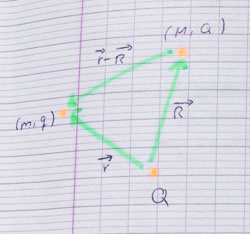
\includegraphics[width=0.4\textwidth]{Skizzen/Anhang2Kopie.jpg}
\end{center}
\caption{}
\end{figure}
$\vec{F}=cqQ\frac{\vec{r}-\vec{R}}{|r-R|^3}$\\
$qQ<0$: anziehend\\
$qQ>0$: abstoßende\\
$c$: Konstante, abhängig von der Einheit Ladung
\end{enumerate}
\end{description}
\subsection{Arbeit und Energie}
\begin{align*}
m\ddot{\vec{r}}\dot{\vec{r}}=\vec{F}\dot{\vec{r}}\\
\frac{d}{dt}(0,5m\dot{\vec{r}}^2)	\Rightarrow\int_{t_1}^{t_2}dt(\frac{d}{dt}(0,5m\dot{\vec{r}}^2))=\int_{t_1}^{t_2}dt\vec{F}\dot{\vec{r}}\\
\Rightarrow T(t_2)-T(t_1)=\int_{t_1}^{t_2}\vec{F}\frac{d\vec{r}}{dt}dt =\int_{t_1}^{t_2}\vec{F}d\vec{r}(t)
\end{align*}
Entlang der Kurve$L$ $\vec{r}(t)$ mit $r(t_1)=r_1...$
\begin{figure}[h]
\begin{center}
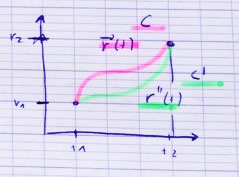
\includegraphics[width=0.4\textwidth]{Skizzen/Anhang2.jpg}
\end{center}
\caption{}
\end{figure}
Wir definieren die am Teilchen geleistete Arbeit entlang $L$ durch $W_e(r_1\rightarrow r_2)=\int_L \vec{F}d\vec{r}=\int_{t_1}^{t_2}\vec{F}\dot{\vec{r}}dt$\\
Wir nennen ein Kraftfeld $\vec{F}$ \underline{konservativ}, wenn $W_e$ nur von $r_1$ und $r_2$, aber nicht vom Weg $r(t)$ abhängt.\\
\begin{description}
\item[Theorem] $\vec{F}(\vec{r})$ konservativ $\Leftrightarrow$ es existiert ein skalares Potential $U(\vec{r})$ mit $\vec{F}(\vec{r})=-\nabla U(\vec{r})$
\begin{align*}
\Leftrightarrow \oint\vec{F}(\vec{r})d\vec{r}=0 \Leftrightarrow\nabla \times\vec{F}=0
\end{align*}
, Kraftfeld ist Wirbelfrei.
\end{description}
Für konservative Kraftfelder gilt: $\int_L F(r)dr=-U(r_2)+U(r_1)=W(r_1\rightarrow r_2)$\\
$\Rightarrow$ $T(t_2)+U(r_2)=T(t_1)+U(r_1)$\\
wir sehen für konservative Kräfte $F=-\nabla U(r)$ folgt:\\
\underline{Energieerhaltung} $E=T+U=0,5m\dot{r}+U(r(t))=const$!\\
denn $\frac{d}{dt}E=m\dot{r}\ddot{r}+\nabla U(r(t))\dot{r}(t)=\dot{r}(t)(m\ddot{r}+\nabla U)=0$ (Newton-Gleichung)
\subsubsection{Beispiele konservativer Kraftfelder}
$F=-\nabla U$\\
\begin{enumerate}
\item $F=F_0 \Rightarrow U(r)=-F_0r$
\item Federkraft $F=-kr \Rightarrow U(r)=0,5f(r\D r)=0,5kr^2$ (harmonischer Oszilator)
\item Coulombkraft, $U(r)=cqQ\frac{1}{|r-R|}$

\subsubsection{Gegenbeispiel}
\item Reibungskraft $F=-\alpha \dot{r}$ konservativ?\\
berechne Arbeit entlang einer geschlossenen Bahn:$\oint Fdr=-\alpha \oint \dot{r}dr=-\alpha \oint \dot{r}^2dt \neq 0, >0$ (außer $\dot{r}=0$)
\end{enumerate}
\subsubsection{Bemerkung}
\begin{enumerate}
\item $E=T+U; T=0,5m\dot{r}^2$ \underline{Kinetische Energie};\\
$U=U(r)$ \underline{potentielle Energie}, nur bis auf additive Konstante festgelegt (definiert das \underline{Energie-Nullniveau})
\begin{figure}[h]
\begin{center}
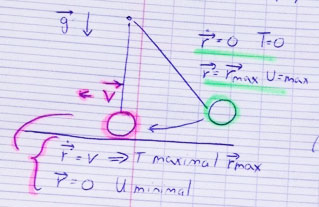
\includegraphics[width=0.4\textwidth]{Skizzen/Anhang1Kopie.jpg}
\end{center}
\caption{}
\end{figure}
\item $E=const$ wichtiger \underline{Energieerhaltungssatz}. (hängt zusammen mit Symmetrien!)
\end{enumerate}
\subsection{Systeme mehreren (N) Teilchen}
\begin{figure}[h]
\begin{center}
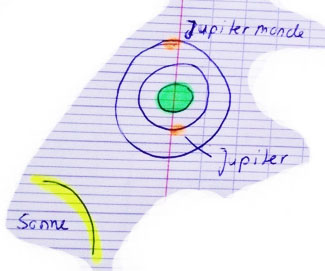
\includegraphics[width=0.4\textwidth]{Skizzen/Anhang1.jpg}
\end{center}
\caption{}
\end{figure}
Dynamik: N Punkteilchen mit Ortsvektoren $r$; $i=1$, $N$ und trägen Massen $m$; es gelten Newtons Gleichungen
\begin{align*}
m_i\ddot{r_i}=F_i (r_1,...r_N,\dot{r_1},...\dot{r_N},t)
\end{align*}
N gekoppelte Diff.-Gl. für die $r_i(t)$; Anfangsbed. $r(0); \dot{r}(0)$ müssen gegeben sein.\\
Häufig: konservative Kräfte: $F_i=-\nabla_i U(r_1,...,r_N)$ es folgt Energieerhaltung (Gesamtenergie).
\begin{align*}
E=\sum^N_{i=1} 0,5m_i\dot{r_i}^2(t)+U(r_1(t),...,r_N(t))=const\\
\nabla_i=\frac{\delta}{\delta r_i}
\end{align*}
häufig setzt sich die Kraft $F_i$ zusammen aus 'äußeren' Kräften $F_i^{(a)}$ und paarweise auftretenden 'inneren' Kräften $F_{ij}$ zwischen den $N$ Teilchen.
\begin{align*}
F_i=F_i^{(a)}(r_i) + \sum^N_{j=1; j\neq i}F_{ij}(r_i,r_j)
\end{align*}
konservative Kräfte: $F_i^{(a)}(r_i)=-\nabla_i U^{(a)}(r_1,...,r_N)$\\
und $F_{ij}=-\nabla_i\sum^N_{j=1; i\neq j}V_{ji}(|r_i-r_j|)$ für abstandsabh. Zweiwechselwirkung ($F_{ij}=-F_{ji}$)\\
es folgt Energieerhaltung in der Form:
\begin{align*}
E=\sum^N_{i=1}0,5m_i\dot{r_i}^2+U^{(a)}(r_1,...,r_N)+0,5\sum^N_{i,j=1; i\neq j}V_{ij}(|r_i-r_j|)
\end{align*}
kin Energie + äußere Pot. Energie + innere Energie
\subsection{N-Teilchenproblem}
\begin{align*}
m_i\ddot{\vec{r_i}}=\vec{F_i^{(a)}}(\vec{r_i})+\sum_{i=1, j\neq i}^{N}\vec{F_{ij}}(\vec{r_i}-\vec{r_j})
\end{align*}
\begin{figure}[h]
	\begin{center}
		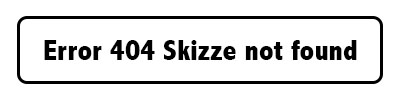
\includegraphics[width=0.4\textwidth]{skizze.jpg}
	\end{center}
	\caption{innere und äußere Kräfte}
\end{figure}
\emph{für konservative Kräfte} 
\begin{flalign}
	\vec{F_i^{(a)}}=-\vec{\nabla_i} U_i(\vec{r_i})\\
	\vec{F_{ij}}=-\vec{\nabla_i}V_{ij}(|\vec{r_i}-\vec{r_j}|)
\end{flalign}
Gesamtenergieerhaltung: $E=T+U^{(a)}+v^{WW}$\\
\paragraph{Bemerkungen:}
	\begin{enumerate}
	\item \emph{Abgeschlossene Systeme} sind solche ohne äußere Kräfte, also \\
		$\vec{F_i^{(a)}}=0, U^{(a)}=\text{const.}$
	\item \emph{Schwerpunkt} des Systems:
	\begin{flalign*}
		\vec{R_{CM}}=\frac{1}{M}\sum_{i=1}^{N}m_i\vec{r_i}, 	& M=\sum_{i}m_i\\
																& \text{Gesamtmasse}
	\end{flalign*}
	\item \emph{Trennung der Energie in Schwerpunkt und Relativteil}:
	\begin{flalign*}
		\dot{\vec{r_i}} =  \dot{\vec{R_{CM}}}+\dot{\vec{\rho_i}} & \text{ Definition von} \vec{\rho_i}\\
		T=\sum_{i=1}^{N}\frac{1}{2}m_i\dot{\vec{r_i}}2=\frac{1}{2}M\dot{\vec{R_{CM}}}^2+\dot{\vec{R_{CM}}}\cdot
		\underbrace{\sum_{i=1}^{N}m_i\dot{\vec{\rho_i}}}_{=0}+\sum_{i=1}^{N}\half m_i\dot{\vec{\rho_i}}^2\\
		\sum_{i=1}^{N}m_i\vec{r_i}=\sum_{i=1}^{N}m:i(\vec{R_{CM}}+\vec{\rho_i})=M\vec{R_{CM}}+\underbrace{\sum_{i=1}^{N}m_i\vec{\rho_i}}_{=0}\\
		T=\underbrace{T_{CM}}_{\half M\dot{\vec{R}}_{CM}^2}+T{rel}
	\end{flalign*}
	\end{enumerate}
für abgeschlossene Systeme
\begin{flalign*}
	E	&=E_{CM}\cdot E_{rel}\\
		&=T_{CM} + (T_{rel}+V^{WW})
\end{flalign*}

\subsection{Impuls und Drehimpuls}
\paragraph{Gesamtimpuls:}
\begin{flalign}
	\vec{P}_{CM}=\sum_{i=1}^{N}m_i\dot{\vec{r}}_i=M\dot{\vec{R}}_{CM}
\end{flalign}
\paragraph{Änderung:}
\begin{flalign}
	\diff{}{t}\vec{P_{CM}}=\sum_{i=1}^{N}(\vec{F_i}^{(a)}+\sum_{j=1; j\neq i}^{N}\vec{F_{ji}})\\
	=\sum_{i=1}^{N}\vec{F_i}^{(a)}+\underbrace{\sum_{i,j=1; i\neq j}^{N}\vec{F_{ji}}}_{=0\text{ (alle Kräfte und ihre Gegenkräfte)}}=\sum_{i=1}^{N}\vec{F_i}^{(a)}
\end{flalign}
\paragraph{Bemerkungen:}
\begin{enumerate}
	\item für abgeschlossene Systeme gilt Gesamtimpulserhaltung:
	\begin{flalign}
		\vec{P_{CM}}(t)=\vec{P_{CM}}(0)=\text{const.}\\
		\text{falls:}\vec{F_i}^{(a)}=0
	\end{flalign}
	\item für $\vec{R_{CM}}$ folgt für abgeschlossene Systeme: 'Schwerpunktsatz'
\\
\begin{flalign}
\vec{R_{cm}}(t)=\vec{R_{CM}}(t_0)+\frac{P{CM}(t_0)}{M}(t-t_0)
\end{flalign}
Schwerpunkt bewegt sich geradlinig-gleichförmig (für abgeschlossene Systeme)
\item Beschreibung der Dynamik ausgedehnter Pbjekte durch Punktteilchen (Schwerpunkt) ist gerechtfertigt
\item $\vec{P_{CM}}=\const$ sehr wichtig für Stoßprozesse gültig für
$\left\{
\begin{array}{cc}
	\text{elastische Stoßprozesse:}	&	E=\const	\\
	\text{inelastischer Stoß:}		&	\text{ein Teil der Enerdie geht über in Verformung}
\end{array}
\right.$
\item häufig Wahl des Schwerpunktsystems $O\rightarrow \vec{R_{CM}}$ (Ursprung) als Bezugssystem
\end{enumerate}
%
\subsubsection{Drehimpuls}
%
\begin{flalign}
\underbrace{\vec{L}=\vec{r}\times\vec{p}}_{\text{(hängt von der Wahl des Ursprungs ab)}}; 	&	\vec{p}=m\dot{\vec{r}}
\end{flalign}
%
\paragraph{zeitliche Änderung:}
%
\begin{flalign}
\diff{}{t}\vec{L}=\underbrace{(\dot{\vec{r}}\times\vec{p})}_{0}+\vec{r}\times\dot{\vec{p}}=\vec{r}\times\vec{F}=:\underbrace{\vec{M}}_{\text{Drehmoment}}\\
\ulcorner \diff{}{t}\vec{p}=\vec{F}, \diff{}{t}\vec{L}=\vec{M} \lrcorner
\end{flalign}
%
\paragraph{für N-Teilchen: Gesamtdrehimpuls}
%
\begin{flalign}
\vec{L_{\ges}}=\sum_{i=1}^{N}\vec{L_i}=\sum_{i=1}^{N}m_i(\vec{r_i}\times\vec{r_i})
\end{flalign}
%
\paragraph{Zeitliche Änderung:}
%
\begin{flalign}
	\diff{}{t}\vec{L}_{\ges}&=\sumni (\vec{r_i}\times\vec{F_i})=\sumni(\vec{r_i}\times\vec{F_i}^{(a)}+\sumij\vec{F_ij})\\
	&\Rightarrow \diff{}{t}\vec{L_{\ges}}=\underbrace{\sumni\vec{M_i}^{(a)}}_{äußeres Drehmoment}+\sumij(\vec{r_i}\times\vec{F_{ij}})\\
	&\Rightarrow \diff{}{t}\vec{L_{\ges}}=\vec{M}^{(a)}=\sumni\vec{M_i}^{(a)}
\end{flalign}
%
\paragraph{Bemerkung:}
%
\begin{enumerate}
	\item für geschlossene Systeme ($\vec{M_i}^{(a)}=0$) gilt \emph{Gesamtdrehimpulserhaltungssatz}:
		\begin{flalign}
			L_{ges}=\sumni \vec{L_i}=\const
		\end{flalign}
	\item Zerlegung in Schwerpunkt und Relativteil: $\vec{r_i}=\vec{R_{CM}}+\vec{\varrho_i}$
	\begin{flalign}
		\vec{L}=\sumni (\vec{r_i}\times\vec{p_i})=\underbrace{\vec{R_{CM}}\times\vec{P_{CM}}}_{\vec{L}_{CM}}+\underbrace{\sumni(\vec{\varrho_i}\times\vec{p_i})}_{\vec{L}_{rel}}
	\end{flalign}
	\item diese Erhaltungssätze für abgeschlossene N-Teilchensysteme gelten:\\
	\begin{flalign*}
		E & & \text{Energie} & & 1\times\\
		\vec{P_{CM}} & & \text{Gesamtimpuls} & & 3\times\\
		\vec{L_{\ges}} & & \text{Gesamtdrehimpuls} & & 3\times
	\end{flalign*}
	\emalign{
		\vec{R_{CM}}(0)=\vec{R_{CM}}(t)-\frac{\vec{P}t}{M} & & \text{Schwerpunktsatz}
		}
	$\Rightarrow$ 10 Erhaltungsgrößen für dynamik eines abgeschlossenen Systems\\
	$\leftrightarrow$ verknüpft mit der Homogenität der Zeit ($t\rightarrow t+t_0$), Homogenität des Raumes ($\vec{r}\rightarrow\vec{r}+\vec{r_0}$), Isotopie des Raumes ($\vec{r}\rightarrow R\vec{r}$)\\
	Galilei-Transformation:
	\begin{flalign*}
		r'&\rightarrow\vec{r}-\vec{v}t\\
		t&\rightarrow t
	\end{flalign*}
	\item für abgeschlossene Systeme gelten die Newtonschen-Gleichungen
	\begin{flalign*}
		& m_i\ddot{\vec{r_i}}=\sumij \vec{F_{ij}}(|r_i-r_j|) & & \text{in IS beim Übergang in IS'} &
	\end{flalign*}
	\begin{flalign*}
		\rightarrow |\vec{r_i}-\vec{r_j}|=|\vec{r_i}'-\vec{r_j}'| & & \text{mit} & & \vec{r_i}'=\vec{_i}+\vec{r_0}-\vec{v}t\\
		& & \text{mit} & & \vec{r_i}'=R\vec{r_i}\\
		\diff{}{t}=\diff{}{t'} & & \text{mit} & & t'=t+t_0\\
		\diff{^2\vec{r}}{t^2}=\diff{'\vec{r}'}{t^2}=\diff{\vec{r}'}{t'^2}
	\end{flalign*}
	\begin{flalign*}
		\Rightarrow\text{in IS' gelten Newtonsche-Bewegungs Gleichungen.}\\
		\Rightarrow m_i \diff{^2\vec{r_i}'}{t'^2}	&=\vec{F_{ij}}'(|\vec{r_i}'-\vec{r_j}'|)\\
		\vec{F}'									&=\vec{F}
	\end{flalign*}
	$\Rightarrow$ Newtonsche Mechanik eines abgeschlossenen Systems ist invariant unter Galilei-Gruppe
\end{enumerate}
%
\subsection{Nicht-Inertialsysteme und Scheinkräfte}
%
Sei ($O,\vec{e_1},\vec{e_2},\vec{e_3}$) IS\\
$\rightarrow$ gehe über zu beschleunigtem (rotierendem) BS\\
$\rightarrow$ mit ($O(t),\vec{e_1}'(t),\vec{e_2}'(t),\vec{e_3}'(t)$)
\begin{enumerate}
	\item Einführung einer zeitabhängigen Rotation:
	\begin{flalign*}
		\vec{e_i}'(t)=R(t)\vec{e_i}\\
		RR^T=\mathds{1}
	\end{flalign*}
	in BS' $\vec{r}'(t)=\sumni x_i'(t)\vec{e_i}'(t)$\\
	für Geschwindigkeit folgt:
	\begin{flalign*}
		& \diff{}{t}(\vec{r}'(t))=\sumni \dot{x}_i'(t)\vec{e_i}'(t)+\sumni x_i'(t)\dot{\vec{e_i}'}(t)=\underbrace{\dot{\vec{r}'}}_{\text{Geschwindigkeit gemessen in BS'}}+\sumni x_i'(t)\dot{\vec{e_i}'}(t)
		\\ 
		\ulcorner
		& \dot{\vec{e_i}'}=\dot{R}(t)\vec{e_i}=\dot{R}R^T\vec{e_i}'
		\lrcorner
		\\
		& \Rightarrow \diff{}{t}\vec{r}'=\vec{V_{BS}}+\sumni x_i'(t)(\dot{R}R^T)\vec{e_i}'
	\end{flalign*}
				\holine
	\begin{flalign*}
		(O,\{\vec{e_i}\})IS\rightarrow(O'(t),\{\vec{e_i}'(t)\})BS'
	\end{flalign*}
	\paragraph*{Beispiel}
	\skizze{Karusselmit zeitabhängiger Drehung}
	Änderung der Basisvektoren:
	\begin{flalign*}
		\diff{}{t}\vec{e_i}'(t)
		& =(\diff{}{t}R)\vec{r_i}=((\diff{}{t}R)R^T)\vec{e_i}'=M\vec{e_i}'\\
		\text{mit }
		M(t) 
		& 
		=(\diff{}{t}R)R^T=-M^T(t)=\begin{pmatrix}
		0	&	-\Omega_3	&	\Omega_2	\\
		\Omega_3	&	0	&	-\Omega_1	\\
		-\Omega_2	&	\Omega_1	&	0	
		\end{pmatrix}
	\end{flalign*}
	Definition von $\vec{\Omega}=\begin{pmatrix}
	\Omega_1\\
	\Omega_2\\
	\Omega_3
	\end{pmatrix}$\\
	wir sehen $M\vec{b}=\vec{\Omega}\times\vec{b}$, Bewegung im rotierenden BS'\\
	\emalign{
		\diff{\vec{r}}{t}=\dot{\vec{r}'}+\vec{\Omega}\times\vec{r}'
		}
	
\end{enumerate}






%{einschub merles mitschriften}